	\section{Цель работы}
		Изучить возможности и особенности инструментальных средств для создания гипертекста (ГТ) и гипертекстовых электронных справочных систем, а также получить навыки работы с ними и разработать электронную справочную систему для собственного программного приложения. 
	\section{Порядок выполенения работы}
	
		\subsection{Help \& Manual}
			\textbf{Help \& Manual} - это инструмент для создания справки, основанный на Windows, опубликованный компанией EC Software, базирующейся в Австрии. Как и многие инструменты для создания справки, Help \& Manual позволяет писателю создавать один исходный текст, который затем преобразует в несколько целевых форматов. Таким образом автор создает исходный текст, используя редактор, встроенный в программу Help \& Manual. Текст, наряду с настройками пользователя для проекта, хранится в файлах XML.
			
			Поддерживаемые форматы выходных данных:
			\begin{itemize}
				\item PDF
				\item Compiled HTML
				\item HTML Web Page
				\item Visual Studio Help
				\item Microsoft Word
				\item eBook 
				\item ePUB e-books
				\item Amazon Kindle e-books
				\item Printed manuals
			\end{itemize}
		
		\subsection{Пример проекта}
		
		Создадим тестовый проект.
			
		\begin{figure*}[h]
			\centering
			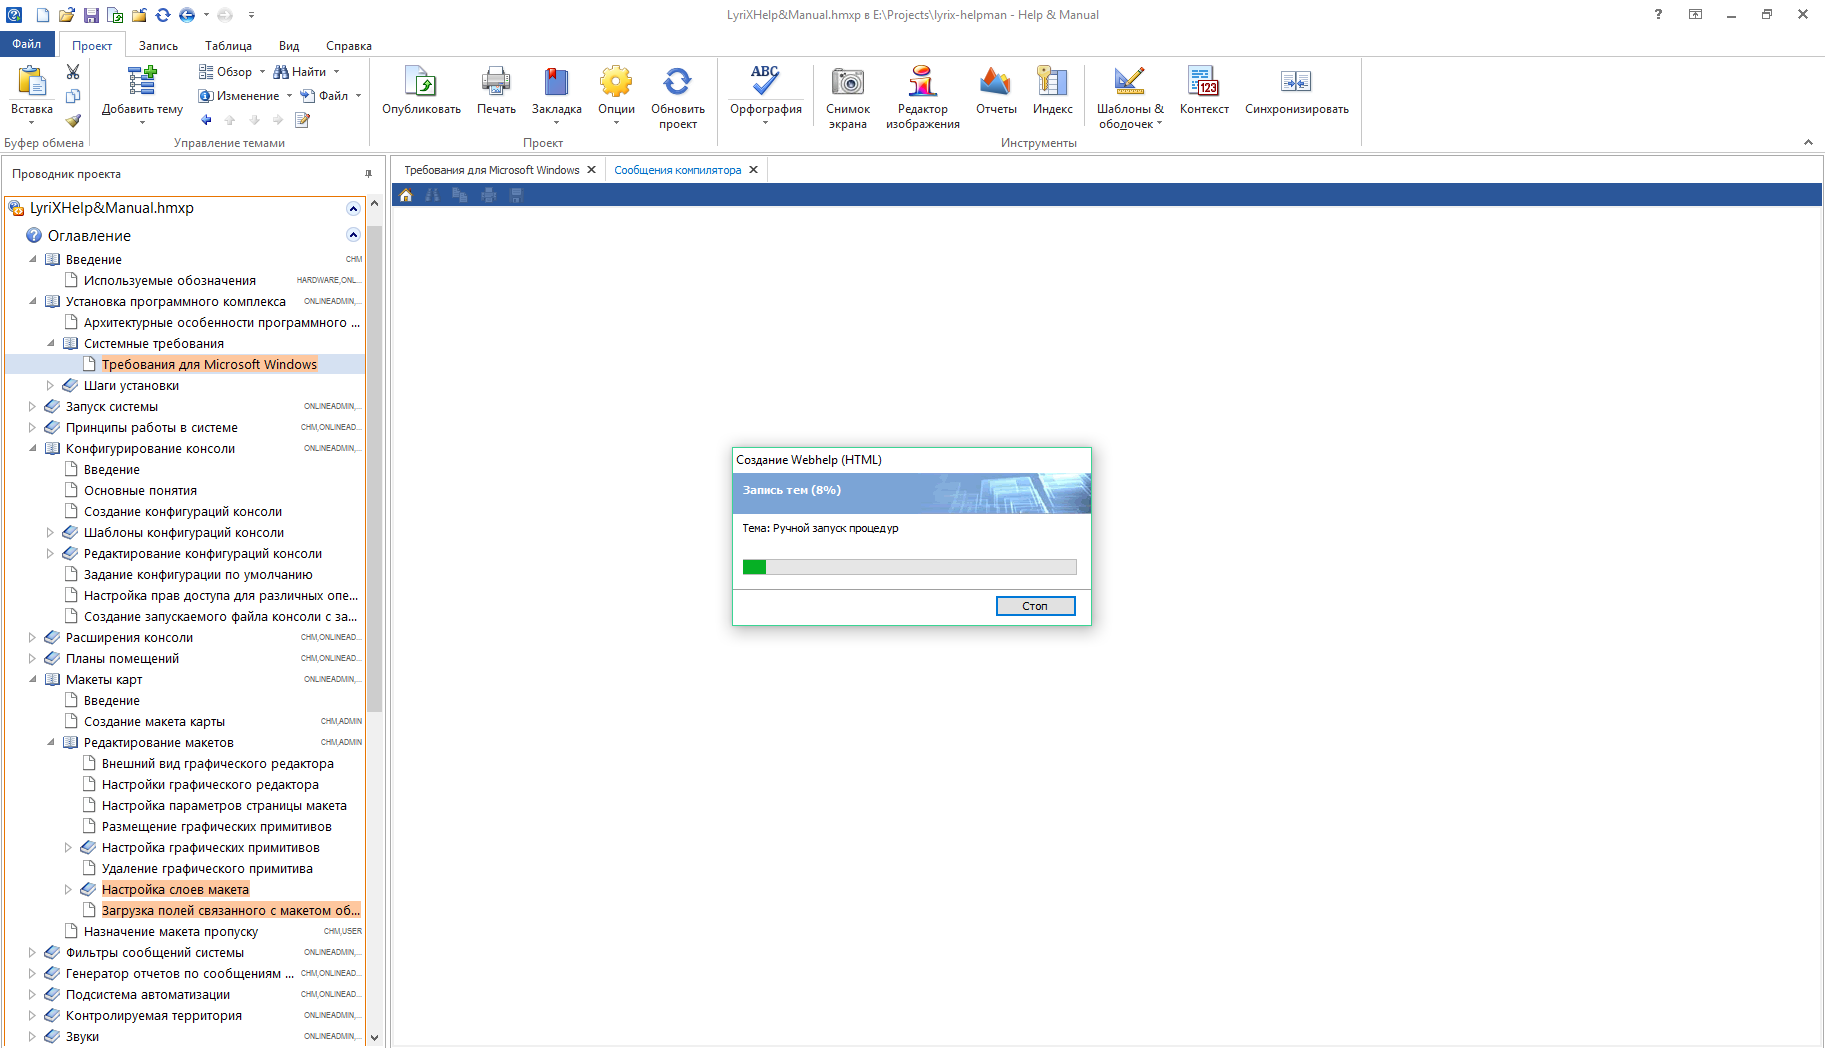
\includegraphics[width=0.7\linewidth]{images/creation}
			\caption{Структура проекта}
			\label{fig:creation}
		\end{figure*}
	
		\FloatBarrier
	
		Для каждого раздела может быть задан тег. С помощью разных комбинаций тегов можно управлять конфигурацией сборки. Это полезно тогда, когда есть несколько версий документа. Например, урезанное руководство для стандартных пользователей и расширенное для администратора.
				
		\begin{figure*}[h]
			\centering
			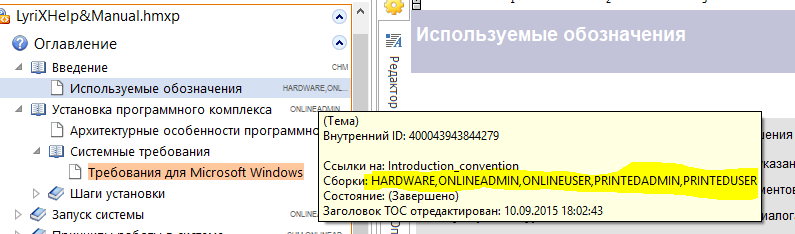
\includegraphics[width=0.7\linewidth]{images/multiple-builds}
			\caption{Множество конфигураций сборки}
			\label{fig:multiple-builds}
		\end{figure*}
	
	
		\FloatBarrier
		Один из вариантов публикации - формат WebHelp. Гипертекст в формате WinHelp реализуется в виде файла с расширением HLP (help-файла). HLP-файл формируется на основе файлов с текстом в формате RTF с помощью специального компилятора.
	
		\begin{figure*}[h]
			\centering
			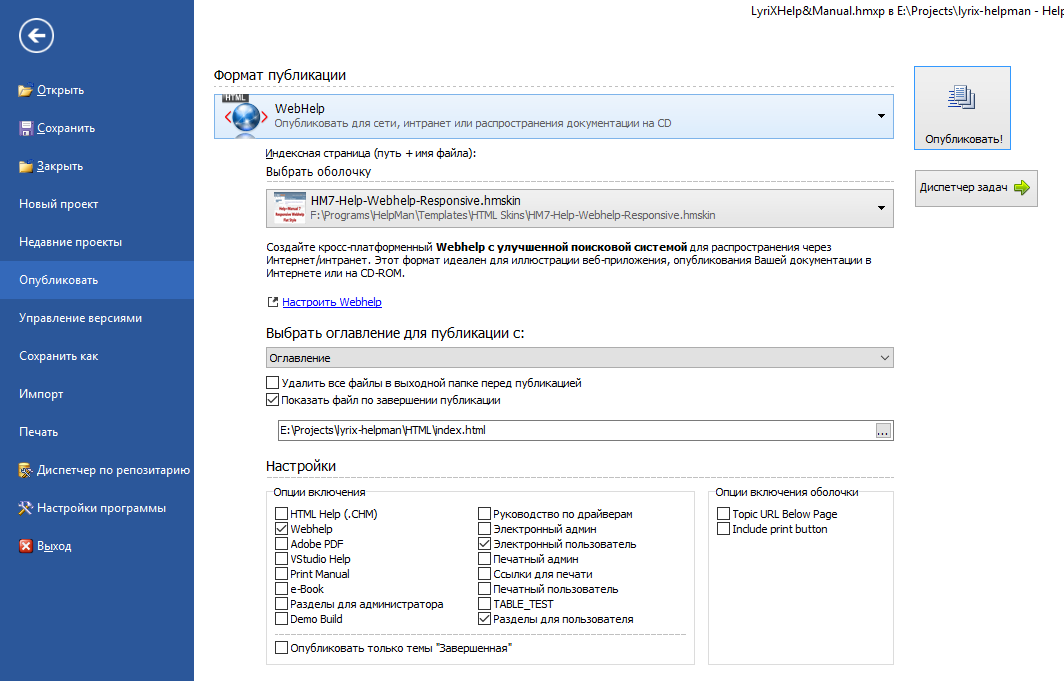
\includegraphics[width=0.7\linewidth]{images/publishing}
			\caption{Публикация в формате WebHelp}
			\label{fig:publishing}
		\end{figure*}
	
		\FloatBarrier
	
		Ниже приведены элементы навигации для такого документа.
	
		\begin{figure*}[h]
			\centering
			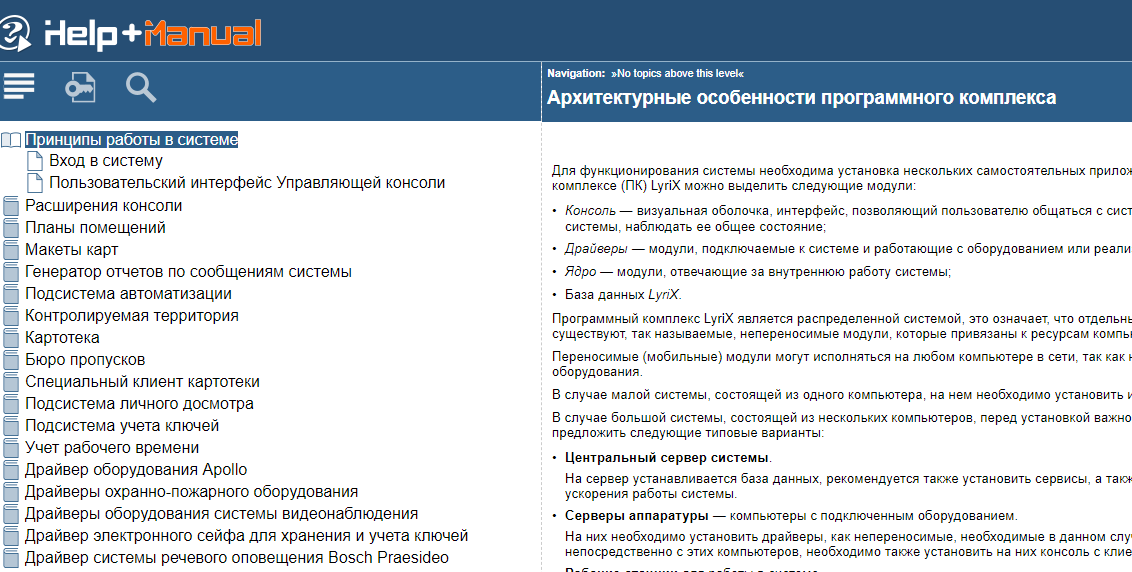
\includegraphics[width=0.7\linewidth]{images/table-of-content}
			\caption{Содержание}
			\label{fig:table-of-content}
		\end{figure*}
		\begin{figure*}[h]
			\centering
			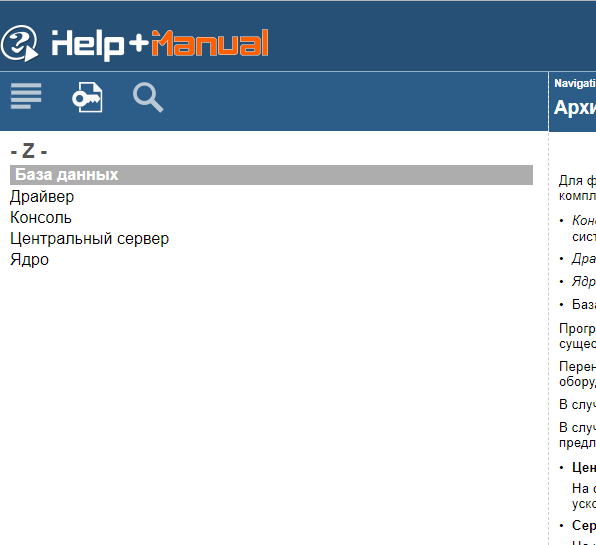
\includegraphics[width=0.7\linewidth]{images/ketword-index}
			\caption{Тезариус}
			\label{fig:ketword-index}
		\end{figure*}
		\begin{figure*}[h]
			\centering
			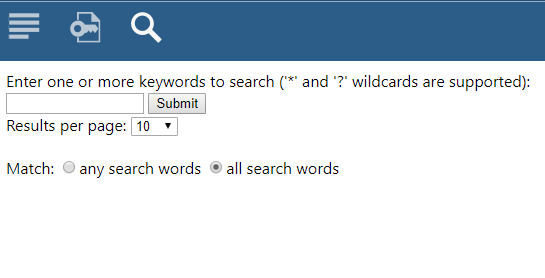
\includegraphics[width=0.7\linewidth]{images/search}
			\caption{Поиск}
			\label{fig:search}
		\end{figure*}
	
		\FloatBarrier
		
		\lstinputlisting[language={XML},caption={Пример страницы <<Введение>>},label={list:example}]{listings/example.xml}
		
	\section{Вывод}
	
	